% !Mode:: "TeX:UTF-8"
% 这个是为了WinEdt设置的,它的默认不是UTF8.
% !TeX root = ../main.tex
% 若xelatex编译非UTF8文件,需在每个文件中指定字符编码;
% main.tex中手动制定了\atemp和\usewhat参数;
\ifx\atempxetex\usewhat
%\XeTeXinputencoding "gbk"
\fi

% \defaultfont
% \appendix
% 
% %%%%%%%%%%%%%%%%%%%%%%%%%%%%%%%%%%%%%%%%%%%%%%%%%%%%%%%%%
% \BiAppChapter{带章节的附录}{Full Appendix}%
% 完整的附录内容,包含章节,公式,图表等
% 
% %%%%%%%%%%%%%%%%%%%%%%%%%%%%%%%%%%%%%%%%%%%%%%%%%%%%%%%%%
% \BiSection{附录节的内容}{Section in Appendix}
% 这是附录的节的内容
% 
% 附录中图的示例:
% \begin{figure}[h]
% \centering
% 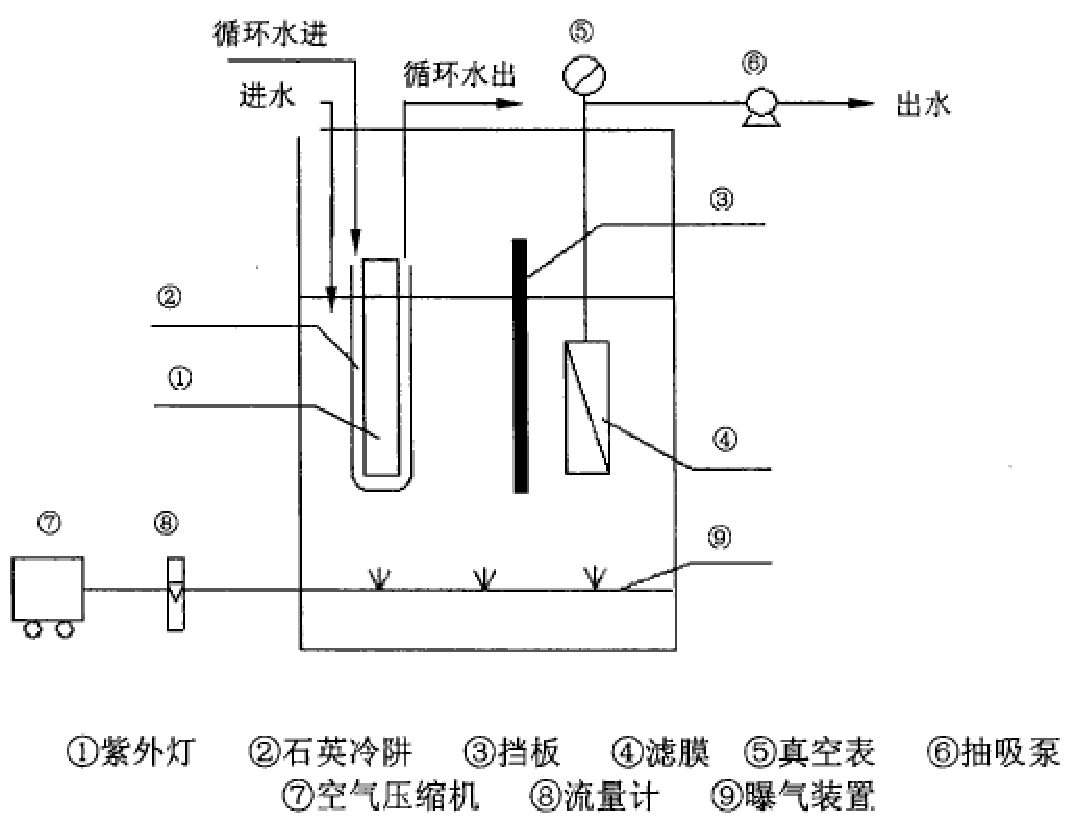
\includegraphics[width = 0.8\textwidth]{golfer}
% \FigureBiCaption{实验装置图~H}{Experiment setup H}
% \label{Figure:Appendix:Example1}
% \end{figure}
% 
% 附录中公式的示例:
% \begin{align}
% a & = b \times c \\
% E & = m c^2
% \end{align}
% 
% %\BiAppChapter{附录二}{appendix 2}
% %\BiAppChapter{附录三}{appendix 3}
